\documentclass[11pt,a4paper,]{article}
\usepackage{lmodern}

\usepackage{amssymb,amsmath}
\usepackage{ifxetex,ifluatex}
\usepackage{fixltx2e} % provides \textsubscript
\ifnum 0\ifxetex 1\fi\ifluatex 1\fi=0 % if pdftex
  \usepackage[T1]{fontenc}
  \usepackage[utf8]{inputenc}
\else % if luatex or xelatex
  \usepackage{unicode-math}
  \defaultfontfeatures{Ligatures=TeX,Scale=MatchLowercase}
\fi
% use upquote if available, for straight quotes in verbatim environments
\IfFileExists{upquote.sty}{\usepackage{upquote}}{}
% use microtype if available
\IfFileExists{microtype.sty}{%
\usepackage[]{microtype}
\UseMicrotypeSet[protrusion]{basicmath} % disable protrusion for tt fonts
}{}
\PassOptionsToPackage{hyphens}{url} % url is loaded by hyperref
\usepackage[unicode=true]{hyperref}
\hypersetup{
            pdfborder={0 0 0},
            breaklinks=true}
\urlstyle{same}  % don't use monospace font for urls
\usepackage{geometry}
\geometry{a4paper, centering, text={16cm,24cm}}
\usepackage[style=authoryear-comp,]{biblatex}
\addbibresource{references.bib}
\usepackage{color}
\usepackage{fancyvrb}
\newcommand{\VerbBar}{|}
\newcommand{\VERB}{\Verb[commandchars=\\\{\}]}
\DefineVerbatimEnvironment{Highlighting}{Verbatim}{commandchars=\\\{\}}
% Add ',fontsize=\small' for more characters per line
\usepackage{framed}
\definecolor{shadecolor}{RGB}{248,248,248}
\newenvironment{Shaded}{\begin{snugshade}}{\end{snugshade}}
\newcommand{\AlertTok}[1]{\textcolor[rgb]{0.94,0.16,0.16}{#1}}
\newcommand{\AnnotationTok}[1]{\textcolor[rgb]{0.56,0.35,0.01}{\textbf{\textit{#1}}}}
\newcommand{\AttributeTok}[1]{\textcolor[rgb]{0.77,0.63,0.00}{#1}}
\newcommand{\BaseNTok}[1]{\textcolor[rgb]{0.00,0.00,0.81}{#1}}
\newcommand{\BuiltInTok}[1]{#1}
\newcommand{\CharTok}[1]{\textcolor[rgb]{0.31,0.60,0.02}{#1}}
\newcommand{\CommentTok}[1]{\textcolor[rgb]{0.56,0.35,0.01}{\textit{#1}}}
\newcommand{\CommentVarTok}[1]{\textcolor[rgb]{0.56,0.35,0.01}{\textbf{\textit{#1}}}}
\newcommand{\ConstantTok}[1]{\textcolor[rgb]{0.00,0.00,0.00}{#1}}
\newcommand{\ControlFlowTok}[1]{\textcolor[rgb]{0.13,0.29,0.53}{\textbf{#1}}}
\newcommand{\DataTypeTok}[1]{\textcolor[rgb]{0.13,0.29,0.53}{#1}}
\newcommand{\DecValTok}[1]{\textcolor[rgb]{0.00,0.00,0.81}{#1}}
\newcommand{\DocumentationTok}[1]{\textcolor[rgb]{0.56,0.35,0.01}{\textbf{\textit{#1}}}}
\newcommand{\ErrorTok}[1]{\textcolor[rgb]{0.64,0.00,0.00}{\textbf{#1}}}
\newcommand{\ExtensionTok}[1]{#1}
\newcommand{\FloatTok}[1]{\textcolor[rgb]{0.00,0.00,0.81}{#1}}
\newcommand{\FunctionTok}[1]{\textcolor[rgb]{0.00,0.00,0.00}{#1}}
\newcommand{\ImportTok}[1]{#1}
\newcommand{\InformationTok}[1]{\textcolor[rgb]{0.56,0.35,0.01}{\textbf{\textit{#1}}}}
\newcommand{\KeywordTok}[1]{\textcolor[rgb]{0.13,0.29,0.53}{\textbf{#1}}}
\newcommand{\NormalTok}[1]{#1}
\newcommand{\OperatorTok}[1]{\textcolor[rgb]{0.81,0.36,0.00}{\textbf{#1}}}
\newcommand{\OtherTok}[1]{\textcolor[rgb]{0.56,0.35,0.01}{#1}}
\newcommand{\PreprocessorTok}[1]{\textcolor[rgb]{0.56,0.35,0.01}{\textit{#1}}}
\newcommand{\RegionMarkerTok}[1]{#1}
\newcommand{\SpecialCharTok}[1]{\textcolor[rgb]{0.00,0.00,0.00}{#1}}
\newcommand{\SpecialStringTok}[1]{\textcolor[rgb]{0.31,0.60,0.02}{#1}}
\newcommand{\StringTok}[1]{\textcolor[rgb]{0.31,0.60,0.02}{#1}}
\newcommand{\VariableTok}[1]{\textcolor[rgb]{0.00,0.00,0.00}{#1}}
\newcommand{\VerbatimStringTok}[1]{\textcolor[rgb]{0.31,0.60,0.02}{#1}}
\newcommand{\WarningTok}[1]{\textcolor[rgb]{0.56,0.35,0.01}{\textbf{\textit{#1}}}}
\usepackage{longtable,booktabs}
% Fix footnotes in tables (requires footnote package)
\IfFileExists{footnote.sty}{\usepackage{footnote}\makesavenoteenv{long table}}{}
\usepackage{graphicx,grffile}
\makeatletter
\def\maxwidth{\ifdim\Gin@nat@width>\linewidth\linewidth\else\Gin@nat@width\fi}
\def\maxheight{\ifdim\Gin@nat@height>\textheight\textheight\else\Gin@nat@height\fi}
\makeatother
% Scale images if necessary, so that they will not overflow the page
% margins by default, and it is still possible to overwrite the defaults
% using explicit options in \includegraphics[width, height, ...]{}
\setkeys{Gin}{width=\maxwidth,height=\maxheight,keepaspectratio}
\IfFileExists{parskip.sty}{%
\usepackage{parskip}
}{% else
\setlength{\parindent}{0pt}
\setlength{\parskip}{6pt plus 2pt minus 1pt}
}
\setlength{\emergencystretch}{3em}  % prevent overfull lines
\providecommand{\tightlist}{%
  \setlength{\itemsep}{0pt}\setlength{\parskip}{0pt}}
\setcounter{secnumdepth}{5}

% set default figure placement to htbp
\makeatletter
\def\fps@figure{htbp}
\makeatother



%% MONASH STUFF

%% CAPTIONS
\RequirePackage{caption}
\DeclareCaptionStyle{italic}[justification=centering]
 {labelfont={bf},textfont={it},labelsep=colon}
\captionsetup[figure]{style=italic,format=hang,singlelinecheck=true}
\captionsetup[table]{style=italic,format=hang,singlelinecheck=true}


%% FONT
\RequirePackage{bera}
\RequirePackage[charter,expert,sfscaled]{mathdesign}
\RequirePackage{fontawesome}

%% HEADERS AND FOOTERS
\RequirePackage{fancyhdr}
\pagestyle{fancy}
\rfoot{\Large\sffamily\raisebox{-0.1cm}{\textbf{\thepage}}}
\makeatletter
\lhead{\textsf{\expandafter{\@title}}}
\makeatother
\rhead{}
\cfoot{}
\setlength{\headheight}{15pt}
\renewcommand{\headrulewidth}{0.4pt}
\renewcommand{\footrulewidth}{0.4pt}
\fancypagestyle{plain}{%
\fancyhf{} % clear all header and footer fields
\fancyfoot[C]{\sffamily\thepage} % except the center
\renewcommand{\headrulewidth}{0pt}
\renewcommand{\footrulewidth}{0pt}}

%% MATHS
\RequirePackage{bm,amsmath}
\allowdisplaybreaks

%% GRAPHICS
\RequirePackage{graphicx}
\setcounter{topnumber}{2}
\setcounter{bottomnumber}{2}
\setcounter{totalnumber}{4}
\renewcommand{\topfraction}{0.85}
\renewcommand{\bottomfraction}{0.85}
\renewcommand{\textfraction}{0.15}
\renewcommand{\floatpagefraction}{0.8}


%\RequirePackage[section]{placeins}

%% SECTION TITLES


%% SECTION TITLES (NEW: Changing sections and subsections color)
\RequirePackage[compact,sf,bf]{titlesec}
\titleformat*{\section}{\Large\sf\bfseries\color[rgb]{0.8, 0.7, 0.1 }}
\titleformat*{\subsection}{\large\sf\bfseries\color[rgb]{0.8, 0.7, 0.1 }}
\titleformat*{\subsubsection}{\sf\bfseries\color[rgb]{0.8, 0.7, 0.1 }}
\titlespacing{\section}{0pt}{2ex}{.5ex}
\titlespacing{\subsection}{0pt}{1.5ex}{0ex}
\titlespacing{\subsubsection}{0pt}{.5ex}{0ex}


%% TITLE PAGE
\def\Date{\number\day}
\def\Month{\ifcase\month\or
 January\or February\or March\or April\or May\or June\or
 July\or August\or September\or October\or November\or December\fi}
\def\Year{\number\year}

%% LINE AND PAGE BREAKING
\sloppy
\clubpenalty = 10000
\widowpenalty = 10000
\brokenpenalty = 10000
\RequirePackage{microtype}

%% PARAGRAPH BREAKS
\setlength{\parskip}{1.4ex}
\setlength{\parindent}{0em}

%% HYPERLINKS
\RequirePackage{xcolor} % Needed for links
\definecolor{darkblue}{rgb}{0,0,.6}
\RequirePackage{url}

\makeatletter
\@ifpackageloaded{hyperref}{}{\RequirePackage{hyperref}}
\makeatother
\hypersetup{
     citecolor=0 0 0,
     breaklinks=true,
     bookmarksopen=true,
     bookmarksnumbered=true,
     linkcolor=darkblue,
     urlcolor=blue,
     citecolor=darkblue,
     colorlinks=true}

\usepackage[showonlyrefs]{mathtools}
\usepackage[no-weekday]{eukdate}

%% BIBLIOGRAPHY

\makeatletter
\@ifpackageloaded{biblatex}{}{\usepackage[style=authoryear-comp, backend=biber, natbib=true]{biblatex}}
\makeatother
\ExecuteBibliographyOptions{bibencoding=utf8,minnames=1,maxnames=3, maxbibnames=99,dashed=false,terseinits=true,giveninits=true,uniquename=false,uniquelist=false,doi=false, isbn=false,url=true,sortcites=false}

\DeclareFieldFormat{url}{\texttt{\url{#1}}}
\DeclareFieldFormat[article]{pages}{#1}
\DeclareFieldFormat[inproceedings]{pages}{\lowercase{pp.}#1}
\DeclareFieldFormat[incollection]{pages}{\lowercase{pp.}#1}
\DeclareFieldFormat[article]{volume}{\mkbibbold{#1}}
\DeclareFieldFormat[article]{number}{\mkbibparens{#1}}
\DeclareFieldFormat[article]{title}{\MakeCapital{#1}}
\DeclareFieldFormat[article]{url}{}
%\DeclareFieldFormat[book]{url}{}
%\DeclareFieldFormat[inbook]{url}{}
%\DeclareFieldFormat[incollection]{url}{}
%\DeclareFieldFormat[inproceedings]{url}{}
\DeclareFieldFormat[inproceedings]{title}{#1}
\DeclareFieldFormat{shorthandwidth}{#1}
%\DeclareFieldFormat{extrayear}{}
% No dot before number of articles
\usepackage{xpatch}
\xpatchbibmacro{volume+number+eid}{\setunit*{\adddot}}{}{}{}
% Remove In: for an article.
\renewbibmacro{in:}{%
  \ifentrytype{article}{}{%
  \printtext{\bibstring{in}\intitlepunct}}}

\AtEveryBibitem{\clearfield{month}}
\AtEveryCitekey{\clearfield{month}}

\makeatletter
\DeclareDelimFormat[cbx@textcite]{nameyeardelim}{\addspace}
\makeatother

\author{\sf\Large\textbf{ Mengyuan YANG}\\ {\sf\large Master of Business Analytics\\[0.5cm]} \sf\Large\textbf{ Zoljargal BATSAIKHAN}\\ {\sf\large Master of Business Analytics\\[0.5cm]} \sf\Large\textbf{ Xinrui WANG}\\ {\sf\large Master of Business Analytics\\[0.5cm]} \sf\Large\textbf{ Xueqi GOH}\\ {\sf\large Master of Business Analytics\\[0.5cm]}}

\date{\sf\Date~\Month~\Year}
\makeatletter
\lfoot{\sf YANG, BATSAIKHAN, WANG, GOH: \@date}
\makeatother


%%%% PAGE STYLE FOR FRONT PAGE OF REPORTS

\makeatletter
\def\organization#1{\gdef\@organization{#1}}
\def\telephone#1{\gdef\@telephone{#1}}
\def\email#1{\gdef\@email{#1}}
\makeatother
  \organization{Monash University}

  \def\name{Our consultancy \newline Mengyuan YANG \&\newline Zoljargal BATSAIKHAN \&\newline Xinrui WANG \&\newline Xueqi GOH}

  \telephone{(03) 9905 2478}

  \email{questions@company.com}                 %NEW: New email addresss

\def\webaddress{\url{http://company.com/stats/consulting/}} %NEW: URl
\def\abn{12 377 614 630}                                    % NEW: ABN
\def\logo{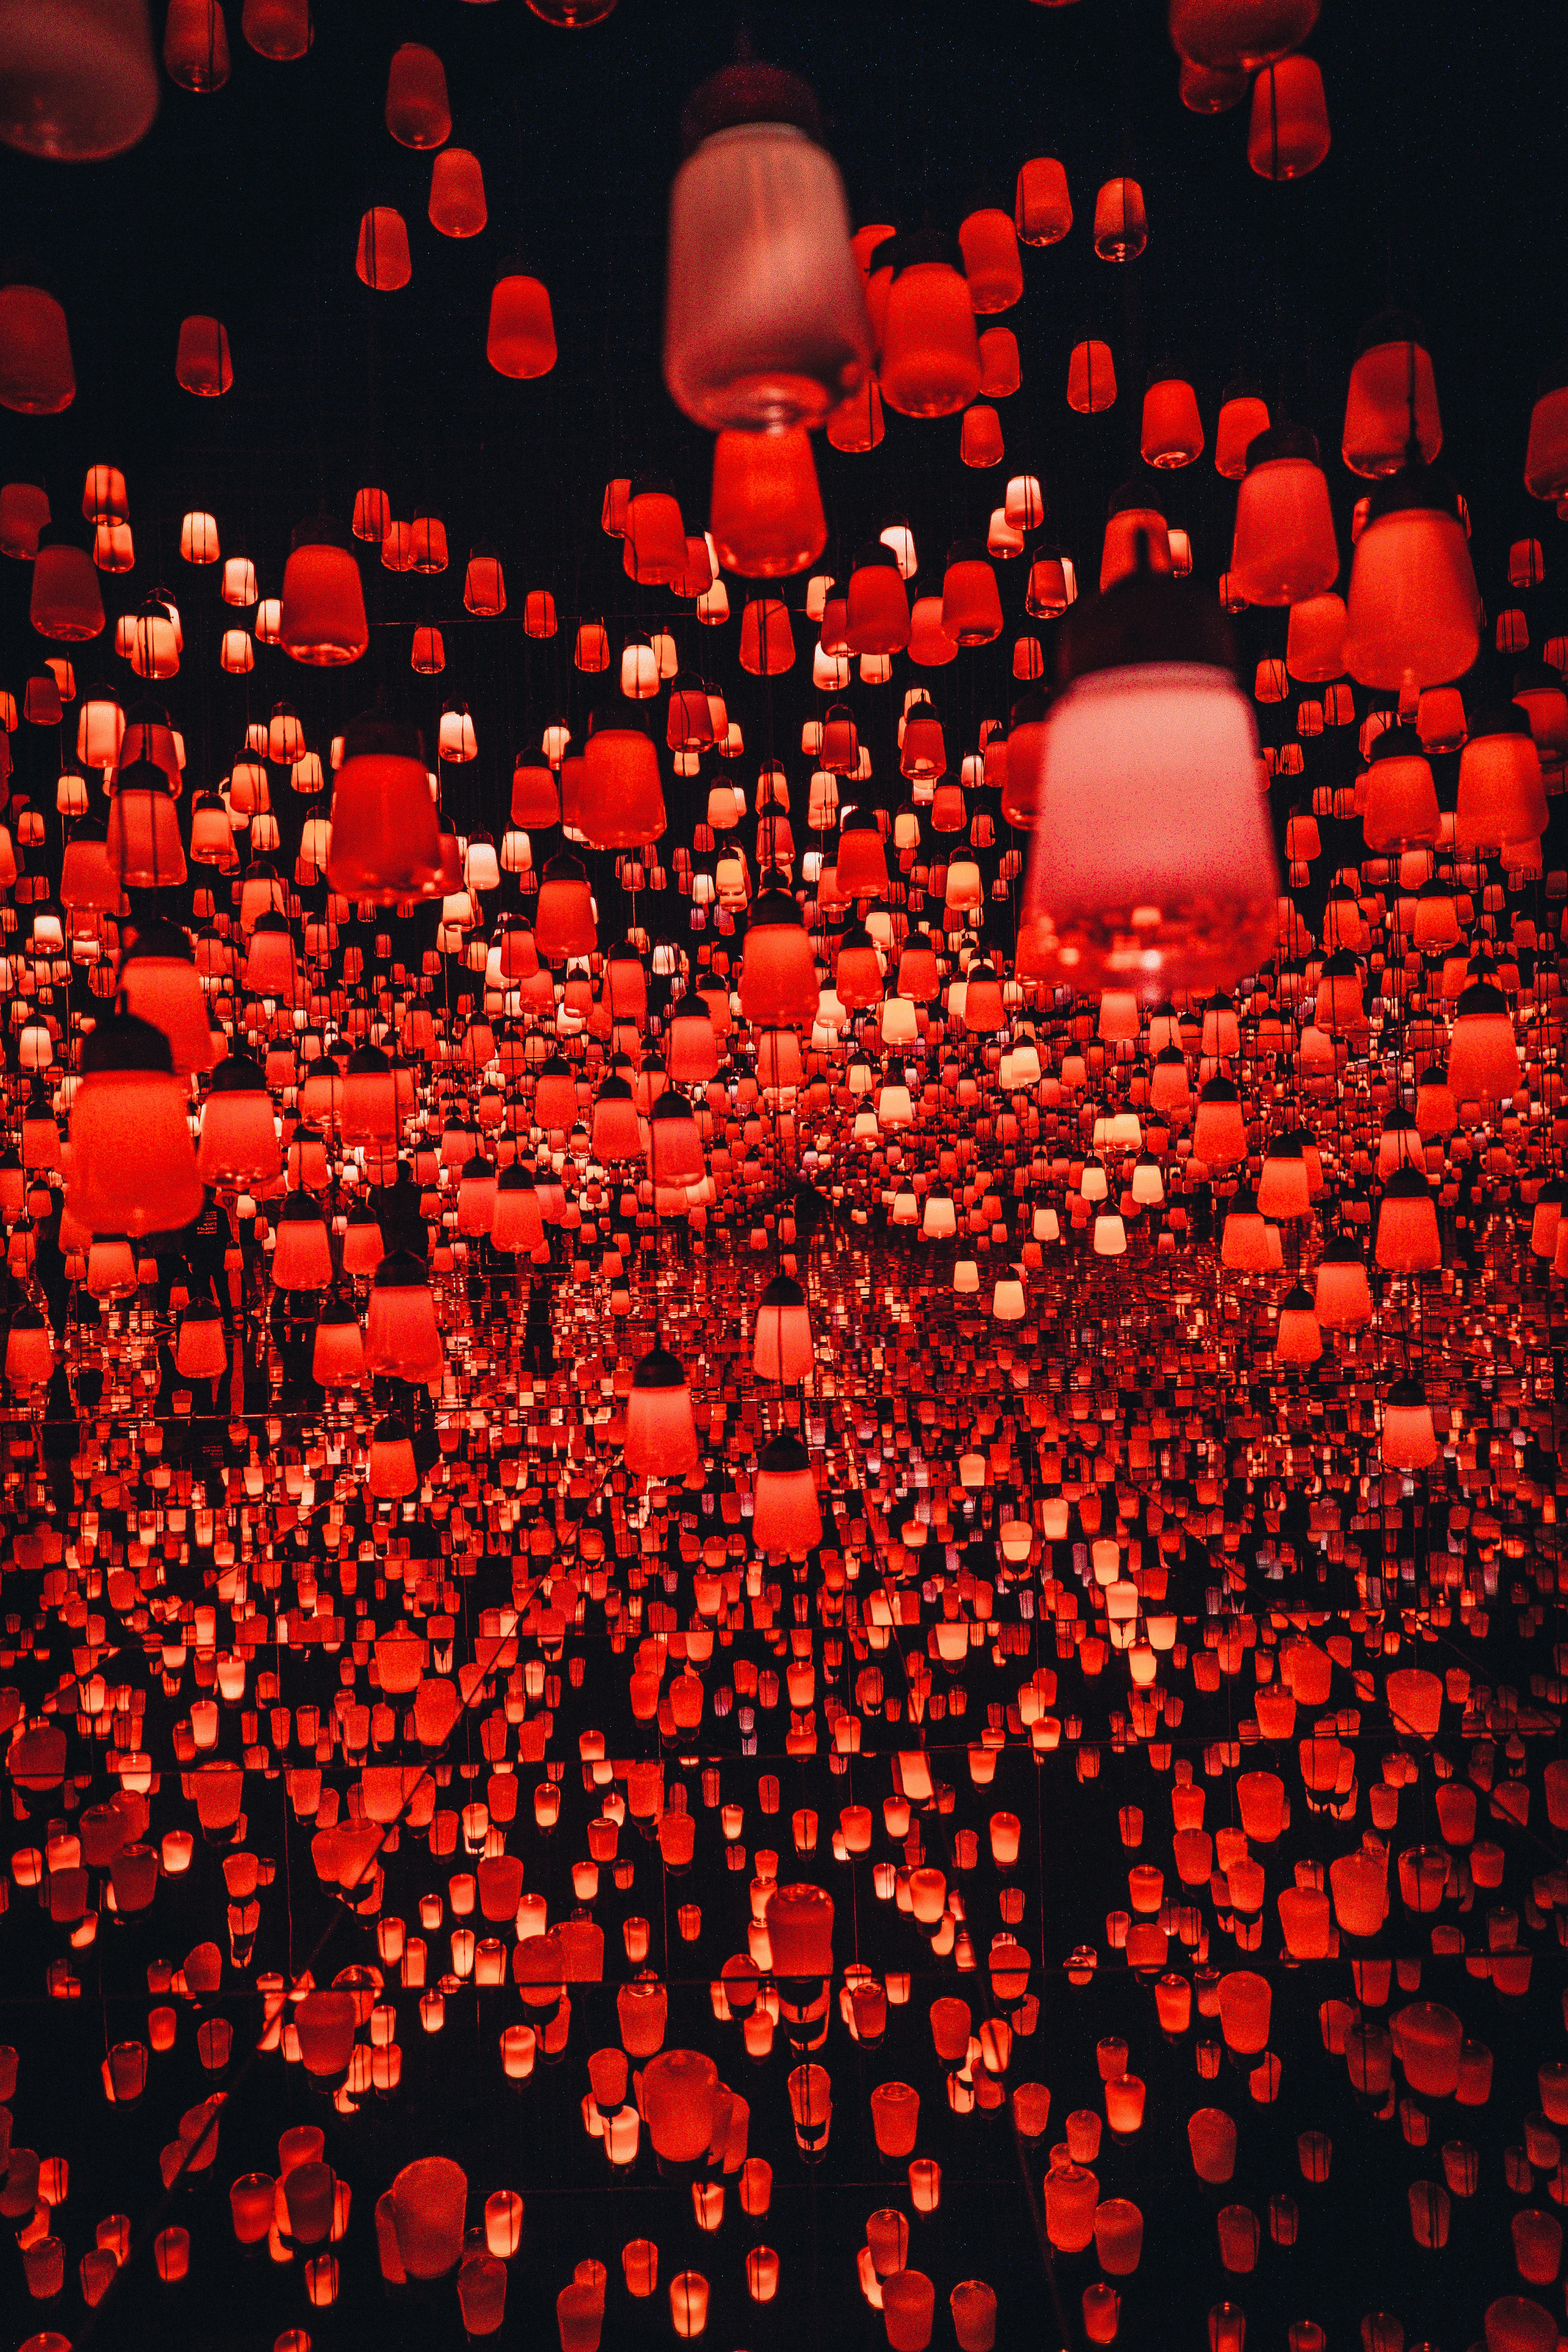
\includegraphics[width=6cm]{Figures/logo}}  %NEW: Changing logo
\def\extraspace{\vspace*{1.6cm}}
\makeatletter
\def\contactdetails{\faicon{phone} & \@telephone \\
                    \faicon{envelope} & \@email}
\makeatother

%%%% FRONT PAGE OF REPORTS

\def\reporttype{Report for}

\long\def\front#1#2#3{
\newpage
\begin{singlespacing}
\thispagestyle{empty}
\vspace*{-1.4cm}
\hspace*{-1.4cm}
\hbox to 16cm{
  \hbox to 6.5cm{\vbox to 14cm{\vbox to 25cm{
    \logo
    \vfill
    \parbox{6.3cm}{\raggedright
      \sf\color[rgb]{0.8, 0.7, 0.1 }    % NEW color 
      {\large\textbf{\name}}\par
      \vspace{.7cm}
      \tabcolsep=0.12cm\sf\small
      \begin{tabular}{@{}ll@{}}\contactdetails
      \end{tabular}
      \vspace*{0.3cm}\par
      ABN: \abn\par
    }
  }\vss}\hss}
  \hspace*{0.2cm}
  \hbox to 1cm{\vbox to 14cm{\rule{4pt}{26.8cm}\vss}\hss\hfill}  %NEW: Thicker line
  \hbox to 10cm{\vbox to 14cm{\vbox to 25cm{   
      \vspace*{3cm}\sf\raggedright
      \parbox{11cm}{\sf\raggedright\baselineskip=1.2cm
         \fontsize{24.88}{30}\color[rgb]{0, 0.29, 0.55}\sf\textbf{#1}}   % NEW: title color blue
      \par
      \vfill
      \large
      \vbox{\parskip=0.8cm #2}\par
      \vspace*{2cm}\par
      \reporttype\\[0.3cm]
      \hbox{#3}%\\[2cm]\
      \vspace*{1cm}
      {\large\sf\textbf{\Date~\Month~\Year}}
   }\vss}
  }}
\end{singlespacing}
\newpage
}

\makeatletter
\def\titlepage{\front{\expandafter{\@title}}{\@author}{\@organization}}
\makeatother

\usepackage{setspace}
\setstretch{1.5}

%% Any special functions or other packages can be loaded here.
\usepackage{booktabs}
\usepackage{longtable}
\usepackage{array}
\usepackage{multirow}
\usepackage{wrapfig}
\usepackage{float}
\usepackage{colortbl}
\usepackage{pdflscape}
\usepackage{tabu}
\usepackage{threeparttable}
\usepackage{threeparttablex}
\usepackage[normalem]{ulem}
\usepackage{makecell}
\usepackage{xcolor}


\begin{document}

{
\setcounter{tocdepth}{2}
\tableofcontents
}
\section*{Introduction}

\begin{Shaded}
\begin{Highlighting}[]
\FunctionTok{excel\_sheets}\NormalTok{(}\StringTok{"data/API\_4\_DS2\_en\_excel\_v2\_2252569.xls"}\NormalTok{)}
\end{Highlighting}
\end{Shaded}

\begin{verbatim}
## [1] "Data"                  "Metadata - Countries"  "Metadata - Indicators"
\end{verbatim}

\begin{Shaded}
\begin{Highlighting}[]
\NormalTok{data\_income }\OtherTok{\textless{}{-}} \FunctionTok{read\_excel}\NormalTok{(}\StringTok{"data/CLASS.xls"}\NormalTok{, }\AttributeTok{range =} \FunctionTok{anchored}\NormalTok{(}\StringTok{"C5"}\NormalTok{, }\AttributeTok{dim =} \FunctionTok{c}\NormalTok{(}\DecValTok{220}\NormalTok{,}\DecValTok{5}\NormalTok{))) }\SpecialCharTok{\%\textgreater{}\%} 
  \FunctionTok{select}\NormalTok{(}\SpecialCharTok{{-}}\NormalTok{X) }\SpecialCharTok{\%\textgreater{}\%} 
  \FunctionTok{filter}\NormalTok{(Economy }\SpecialCharTok{!=} \StringTok{"x"}\NormalTok{)}
\end{Highlighting}
\end{Shaded}

\begin{Shaded}
\begin{Highlighting}[]
\NormalTok{df}\OtherTok{\textless{}{-}} \FunctionTok{read\_excel}\NormalTok{(}\StringTok{"Data/API\_4\_DS2\_en\_excel\_v2\_2252569.xls"}\NormalTok{, }\AttributeTok{sheet =} \DecValTok{1}\NormalTok{, }\AttributeTok{range =} \StringTok{"A4:BM42772"}\NormalTok{) }\SpecialCharTok{\%\textgreater{}\%} 
  \FunctionTok{select}\NormalTok{(}\StringTok{"Country Name"}\NormalTok{, }
         \StringTok{"Country Code"}\NormalTok{,}
         \StringTok{"Indicator Name"}\NormalTok{, }
         \StringTok{"2000"}\SpecialCharTok{:}\StringTok{"2019"}\NormalTok{) }\SpecialCharTok{\%\textgreater{}\%} 
  \FunctionTok{rename}\NormalTok{(}\StringTok{"country\_name"} \OtherTok{=} \StringTok{"Country Name"}\NormalTok{,}
         \StringTok{"indicator"} \OtherTok{=} \StringTok{"Indicator Name"}\NormalTok{,}
         \StringTok{"country\_code"} \OtherTok{=} \StringTok{"Country Code"}\NormalTok{)}
\end{Highlighting}
\end{Shaded}

\begin{Shaded}
\begin{Highlighting}[]
\NormalTok{df }\SpecialCharTok{\%\textgreater{}\%}
  \FunctionTok{group\_by}\NormalTok{(country\_name) }\SpecialCharTok{\%\textgreater{}\%}
  \FunctionTok{miss\_var\_summary}\NormalTok{() }\SpecialCharTok{\%\textgreater{}\%} 
  \FunctionTok{arrange}\NormalTok{(}\SpecialCharTok{{-}}\NormalTok{pct\_miss)}
\end{Highlighting}
\end{Shaded}

\begin{verbatim}
## # A tibble: 5,808 x 4
## # Groups:   country_name [264]
##    country_name  variable n_miss pct_miss
##    <chr>         <chr>     <int>    <dbl>
##  1 Faroe Islands 2000        162      100
##  2 Faroe Islands 2001        162      100
##  3 Faroe Islands 2002        162      100
##  4 Faroe Islands 2003        162      100
##  5 Faroe Islands 2004        162      100
##  6 Faroe Islands 2005        162      100
##  7 Faroe Islands 2006        162      100
##  8 Faroe Islands 2007        162      100
##  9 Faroe Islands 2008        162      100
## 10 Faroe Islands 2009        162      100
## # ... with 5,798 more rows
\end{verbatim}

\begin{Shaded}
\begin{Highlighting}[]
\NormalTok{df\_filter }\OtherTok{\textless{}{-}}\NormalTok{ df }\SpecialCharTok{\%\textgreater{}\%} 
  \FunctionTok{filter}\NormalTok{(}\SpecialCharTok{!}\NormalTok{(country\_name }\SpecialCharTok{\%in\%} \FunctionTok{c}\NormalTok{(}\StringTok{"Faroe Islands"}\NormalTok{,}
                          \StringTok{"Greenland"}\NormalTok{,}
                          \StringTok{"Isle of Man"}\NormalTok{,}
                          \StringTok{"Not classified"}\NormalTok{,}
                          \StringTok{"St. Martin (French part)"}\NormalTok{,}
                          \StringTok{"Northern Mariana Islands"}\NormalTok{,}
                          \StringTok{"Kosovo"}\NormalTok{,}
                          \StringTok{"American Samoa"}\NormalTok{,}
                          \StringTok{"Gibraltar"}\NormalTok{,}
                          \StringTok{"Sint Maarten (Dutch part)"}\NormalTok{,}
                          \StringTok{"Turks and Caicos Islands"}\NormalTok{,}
                          \StringTok{"Channel Islands"}\NormalTok{,}
                          \StringTok{"Guam"}\NormalTok{,}
                          \StringTok{"French Polynesia"}\NormalTok{,}
                          \StringTok{"Curacao"}\NormalTok{,}
                          \StringTok{"New Caledonia"}\NormalTok{,}
                          \StringTok{"Virgin Islands (U.S.)"}\NormalTok{,}
                          \StringTok{"Nauru"}\NormalTok{,}
                          \StringTok{"Palau"}\NormalTok{,}
                          \StringTok{"Somalia"}\NormalTok{,}
                          \StringTok{"Guinea{-}Bissau"}\NormalTok{)))}
\end{Highlighting}
\end{Shaded}

\begin{Shaded}
\begin{Highlighting}[]
\NormalTok{data\_joined }\OtherTok{\textless{}{-}}\NormalTok{ df\_filter }\SpecialCharTok{\%\textgreater{}\%} 
    \FunctionTok{left\_join}\NormalTok{(data\_income, }\AttributeTok{by =} \FunctionTok{c}\NormalTok{(}\StringTok{"country\_name"} \OtherTok{=} \StringTok{"Economy"}\NormalTok{,}
                                \StringTok{"country\_code"} \OtherTok{=} \StringTok{"Code"}\NormalTok{)) }
\end{Highlighting}
\end{Shaded}

\section*{Mengyun}

\section*{Zoljargal}

\section*{Xinrui}

\section*{Xueqi}

\begin{Shaded}
\begin{Highlighting}[]
\NormalTok{df\_xq }\OtherTok{\textless{}{-}}\NormalTok{ data\_joined }\SpecialCharTok{\%\textgreater{}\%}
   \FunctionTok{pivot\_longer}\NormalTok{(}\AttributeTok{cols =} \FunctionTok{c}\NormalTok{(}\StringTok{"2000"}\SpecialCharTok{:}\StringTok{"2019"}\NormalTok{),}
               \AttributeTok{names\_to =} \StringTok{"year"}\NormalTok{,}
               \AttributeTok{values\_to =} \StringTok{"value"}\NormalTok{) }\SpecialCharTok{\%\textgreater{}\%}
\NormalTok{ dplyr}\SpecialCharTok{::}\FunctionTok{filter}\NormalTok{(}\FunctionTok{str\_detect}\NormalTok{(indicator, }\StringTok{\textquotesingle{}Pupil{-}teacher ratio\textquotesingle{}}\NormalTok{) }\SpecialCharTok{\&} \SpecialCharTok{!}\FunctionTok{str\_detect}\NormalTok{(value, }\StringTok{"NA"}\NormalTok{) }\SpecialCharTok{\&} \SpecialCharTok{!}\FunctionTok{str\_detect}\NormalTok{(Region, }\StringTok{"NA"}\NormalTok{)) }\SpecialCharTok{\%\textgreater{}\%}
 \FunctionTok{group\_by}\NormalTok{(Region) }
  
\NormalTok{p1 }\OtherTok{\textless{}{-}}\NormalTok{ df\_xq }\SpecialCharTok{\%\textgreater{}\%}
 \FunctionTok{ggplot}\NormalTok{(}\FunctionTok{aes}\NormalTok{(}\AttributeTok{x =}\NormalTok{ year,}
            \AttributeTok{y =}\NormalTok{ value,}
         \AttributeTok{fill =}\NormalTok{ indicator)) }\SpecialCharTok{+}
  \FunctionTok{geom\_col}\NormalTok{(}\AttributeTok{position =} \StringTok{"dodge"}\NormalTok{, }\AttributeTok{width =} \FloatTok{0.7}\NormalTok{) }\SpecialCharTok{+}
  \FunctionTok{theme\_bw}\NormalTok{() }\SpecialCharTok{+}
  \FunctionTok{theme}\NormalTok{(}\AttributeTok{axis.text.x =} \FunctionTok{element\_text}\NormalTok{(}\AttributeTok{angle =} \DecValTok{60}\NormalTok{, }\AttributeTok{vjust =} \FloatTok{0.5}\NormalTok{, }\AttributeTok{hjust=}\FloatTok{0.5}\NormalTok{)) }\SpecialCharTok{+}
  \FunctionTok{scale\_fill\_brewer}\NormalTok{(}\AttributeTok{palette =} \StringTok{"Paired"}\NormalTok{) }\SpecialCharTok{+}
  \FunctionTok{labs}\NormalTok{(}\AttributeTok{x =} \StringTok{"Year"}\NormalTok{,}
       \AttributeTok{y =} \StringTok{\textquotesingle{}Pupil{-}teacher ratio\textquotesingle{}}\NormalTok{,}
       \AttributeTok{fill =} \StringTok{\textquotesingle{}Pupil{-}teacher ratio\textquotesingle{}}\NormalTok{) }\SpecialCharTok{+}
  \FunctionTok{ggtitle}\NormalTok{(}\StringTok{"Worldwide Region Pupil{-}teacher Ratio between 2000{-}2019"}\NormalTok{) }\SpecialCharTok{+}
  \FunctionTok{facet\_wrap}\NormalTok{( }\SpecialCharTok{\textasciitilde{}}\NormalTok{ Region,}
              \AttributeTok{scales =} \StringTok{\textquotesingle{}free\textquotesingle{}}\NormalTok{,}
              \AttributeTok{strip.position =} \StringTok{\textquotesingle{}right\textquotesingle{}}\NormalTok{)}
\NormalTok{p1}
\end{Highlighting}
\end{Shaded}

\includegraphics{report_files/figure-latex/unnamed-chunk-7-1.pdf}

\section*{Conclusion}

\printbibliography

\end{document}
